%% bare_conf.tex
%% V1.4b
%% 2015/08/26
%% by Michael Shell
%% See:
%% http://www.michaelshell.org/
%% for current contact information.
%%
%% This is a skeleton file demonstrating the use of IEEEtran.cls
%% (requires IEEEtran.cls version 1.8b or later) with an IEEE
%% conference paper.
%%
%% Support sites:
%% http://www.michaelshell.org/tex/ieeetran/
%% http://www.ctan.org/pkg/ieeetran
%% and
%% http://www.ieee.org/

%%*************************************************************************
%% Legal Notice:
%% This code is offered as-is without any warranty either expressed or
%% implied; without even the implied warranty of MERCHANTABILITY or
%% FITNESS FOR A PARTICULAR PURPOSE! 
%% User assumes all risk.
%% In no event shall the IEEE or any contributor to this code be liable for
%% any damages or losses, including, but not limited to, incidental,
%% consequential, or any other damages, resulting from the use or misuse
%% of any information contained here.
%%
%% All comments are the opinions of their respective authors and are not
%% necessarily endorsed by the IEEE.
%%
%% This work is distributed under the LaTeX Project Public License (LPPL)
%% ( http://www.latex-project.org/ ) version 1.3, and may be freely used,
%% distributed and modified. A copy of the LPPL, version 1.3, is included
%% in the base LaTeX documentation of all distributions of LaTeX released
%% 2003/12/01 or later.
%% Retain all contribution notices and credits.
%% ** Modified files should be clearly indicated as such, including  **
%% ** renaming them and changing author support contact information. **
%%*************************************************************************


% *** Authors should verify (and, if needed, correct) their LaTeX system  ***
% *** with the testflow diagnostic prior to trusting their LaTeX platform ***
% *** with production work. The IEEE's font choices and paper sizes can   ***
% *** trigger bugs that do not appear when using other class files.       ***                          
% The testflow support page is at:
% http://www.michaelshell.org/tex/testflow/

\documentclass[conference]{IEEEtran}
% Some Computer Society conferences also require the compsoc mode option,
% but others use the standard conference format.
%
% If IEEEtran.cls has not been installed into the LaTeX system files,
% manually specify the path to it like:
% \documentclass[conference]{../sty/IEEEtran}

\usepackage{booktabs}
\newcommand{\ra}[1]{\renewcommand{\arraystretch}{#1}}

\usepackage[usenames,dvipsnames]{color}
\newcommand{\todo}[1]
  {{\scriptsize \textbf{\color{red} {#1}}}}



% Some very useful LaTeX packages include:
% (uncomment the ones you want to load)


% *** MISC UTILITY PACKAGES ***
%
%\usepackage{ifpdf}
% Heiko Oberdiek's ifpdf.sty is very useful if you need conditional
% compilation based on whether the output is pdf or dvi.
% usage:
% \ifpdf
%   % pdf code
% \else
%   % dvi code
% \fi
% The latest version of ifpdf.sty can be obtained from:
% http://www.ctan.org/pkg/ifpdf
% Also, note that IEEEtran.cls V1.7 and later provides a builtin
% \ifCLASSINFOpdf conditional that works the same way.
% When switching from latex to pdflatex and vice-versa, the compiler may
% have to be run twice to clear warning/error messages.


\usepackage{listings}



% *** CITATION PACKAGES ***
%
\usepackage{cite}
% cite.sty was written by Donald Arseneau
% V1.6 and later of IEEEtran pre-defines the format of the cite.sty package
% \cite{} output to follow that of the IEEE. Loading the cite package will
% result in citation numbers being automatically sorted and properly
% "compressed/ranged". e.g., [1], [9], [2], [7], [5], [6] without using
% cite.sty will become [1], [2], [5]--[7], [9] using cite.sty. cite.sty's
% \cite will automatically add leading space, if needed. Use cite.sty's
% noadjust option (cite.sty V3.8 and later) if you want to turn this off
% such as if a citation ever needs to be enclosed in parenthesis.
% cite.sty is already installed on most LaTeX systems. Be sure and use
% version 5.0 (2009-03-20) and later if using hyperref.sty.
% The latest version can be obtained at:
% http://www.ctan.org/pkg/cite
% The documentation is contained in the cite.sty file itself.






% *** GRAPHICS RELATED PACKAGES ***
%
\ifCLASSINFOpdf
   \usepackage[pdftex]{graphicx}
  % declare the path(s) where your graphic files are
   \graphicspath{{images/}}
  % and their extensions so you won't have to specify these with
  % every instance of \includegraphics
   \DeclareGraphicsExtensions{.pdf,.jpeg,.png, .jpg}
\else
  % or other class option (dvipsone, dvipdf, if not using dvips). graphicx
  % will default to the driver specified in the system graphics.cfg if no
  % driver is specified.
  % \usepackage[dvips]{graphicx}
  % declare the path(s) where your graphic files are
  % \graphicspath{{../eps/}}
  % and their extensions so you won't have to specify these with
  % every instance of \includegraphics
  % \DeclareGraphicsExtensions{.eps}
\fi
% graphicx was written by David Carlisle and Sebastian Rahtz. It is
% required if you want graphics, photos, etc. graphicx.sty is already
% installed on most LaTeX systems. The latest version and documentation
% can be obtained at: 
% http://www.ctan.org/pkg/graphicx
% Another good source of documentation is "Using Imported Graphics in
% LaTeX2e" by Keith Reckdahl which can be found at:
% http://www.ctan.org/pkg/epslatex
%
% latex, and pdflatex in dvi mode, support graphics in encapsulated
% postscript (.eps) format. pdflatex in pdf mode supports graphics
% in .pdf, .jpeg, .png and .mps (metapost) formats. Users should ensure
% that all non-photo figures use a vector format (.eps, .pdf, .mps) and
% not a bitmapped formats (.jpeg, .png). The IEEE frowns on bitmapped formats
% which can result in "jaggedy"/blurry rendering of lines and letters as
% well as large increases in file sizes.
%
% You can find documentation about the pdfTeX application at:
% http://www.tug.org/applications/pdftex





% *** MATH PACKAGES ***
%
\usepackage{amsmath}
% A popular package from the American Mathematical Society that provides
% many useful and powerful commands for dealing with mathematics.
%
% Note that the amsmath package sets \interdisplaylinepenalty to 10000
% thus preventing page breaks from occurring within multiline equations. Use:
%\interdisplaylinepenalty=2500
% after loading amsmath to restore such page breaks as IEEEtran.cls normally
% does. amsmath.sty is already installed on most LaTeX systems. The latest
% version and documentation can be obtained at:
% http://www.ctan.org/pkg/amsmath





% *** SPECIALIZED LIST PACKAGES ***
%
%\usepackage{algorithmic}
% algorithmic.sty was written by Peter Williams and Rogerio Brito.
% This package provides an algorithmic environment fo describing algorithms.
% You can use the algorithmic environment in-text or within a figure
% environment to provide for a floating algorithm. Do NOT use the algorithm
% floating environment provided by algorithm.sty (by the same authors) or
% algorithm2e.sty (by Christophe Fiorio) as the IEEE does not use dedicated
% algorithm float types and packages that provide these will not provide
% correct IEEE style captions. The latest version and documentation of
% algorithmic.sty can be obtained at:
% http://www.ctan.org/pkg/algorithms
% Also of interest may be the (relatively newer and more customizable)
% algorithmicx.sty package by Szasz Janos:
% http://www.ctan.org/pkg/algorithmicx




% *** ALIGNMENT PACKAGES ***
%
%\usepackage{array}
% Frank Mittelbach's and David Carlisle's array.sty patches and improves
% the standard LaTeX2e array and tabular environments to provide better
% appearance and additional user controls. As the default LaTeX2e table
% generation code is lacking to the point of almost being broken with
% respect to the quality of the end results, all users are strongly
% advised to use an enhanced (at the very least that provided by array.sty)
% set of table tools. array.sty is already installed on most systems. The
% latest version and documentation can be obtained at:
% http://www.ctan.org/pkg/array


% IEEEtran contains the IEEEeqnarray family of commands that can be used to
% generate multiline equations as well as matrices, tables, etc., of high
% quality.




% *** SUBFIGURE PACKAGES ***
%\ifCLASSOPTIONcompsoc
%  \usepackage[caption=false,font=normalsize,labelfont=sf,textfont=sf]{subfig}
%\else
%  \usepackage[caption=false,font=footnotesize]{subfig}
%\fi
% subfig.sty, written by Steven Douglas Cochran, is the modern replacement
% for subfigure.sty, the latter of which is no longer maintained and is
% incompatible with some LaTeX packages including fixltx2e. However,
% subfig.sty requires and automatically loads Axel Sommerfeldt's caption.sty
% which will override IEEEtran.cls' handling of captions and this will result
% in non-IEEE style figure/table captions. To prevent this problem, be sure
% and invoke subfig.sty's "caption=false" package option (available since
% subfig.sty version 1.3, 2005/06/28) as this is will preserve IEEEtran.cls
% handling of captions.
% Note that the Computer Society format requires a larger sans serif font
% than the serif footnote size font used in traditional IEEE formatting
% and thus the need to invoke different subfig.sty package options depending
% on whether compsoc mode has been enabled.
%
% The latest version and documentation of subfig.sty can be obtained at:
% http://www.ctan.org/pkg/subfig




% *** FLOAT PACKAGES ***
%
%\usepackage{fixltx2e}
% fixltx2e, the successor to the earlier fix2col.sty, was written by
% Frank Mittelbach and David Carlisle. This package corrects a few problems
% in the LaTeX2e kernel, the most notable of which is that in current
% LaTeX2e releases, the ordering of single and double column floats is not
% guaranteed to be preserved. Thus, an unpatched LaTeX2e can allow a
% single column figure to be placed prior to an earlier double column
% figure.
% Be aware that LaTeX2e kernels dated 2015 and later have fixltx2e.sty's
% corrections already built into the system in which case a warning will
% be issued if an attempt is made to load fixltx2e.sty as it is no longer
% needed.
% The latest version and documentation can be found at:
% http://www.ctan.org/pkg/fixltx2e


%\usepackage{stfloats}
% stfloats.sty was written by Sigitas Tolusis. This package gives LaTeX2e
% the ability to do double column floats at the bottom of the page as well
% as the top. (e.g., "\begin{figure*}[!b]" is not normally possible in
% LaTeX2e). It also provides a command:
%\fnbelowfloat
% to enable the placement of footnotes below bottom floats (the standard
% LaTeX2e kernel puts them above bottom floats). This is an invasive package
% which rewrites many portions of the LaTeX2e float routines. It may not work
% with other packages that modify the LaTeX2e float routines. The latest
% version and documentation can be obtained at:
% http://www.ctan.org/pkg/stfloats
% Do not use the stfloats baselinefloat ability as the IEEE does not allow
% \baselineskip to stretch. Authors submitting work to the IEEE should note
% that the IEEE rarely uses double column equations and that authors should try
% to avoid such use. Do not be tempted to use the cuted.sty or midfloat.sty
% packages (also by Sigitas Tolusis) as the IEEE does not format its papers in
% such ways.
% Do not attempt to use stfloats with fixltx2e as they are incompatible.
% Instead, use Morten Hogholm'a dblfloatfix which combines the features
% of both fixltx2e and stfloats:
%
% \usepackage{dblfloatfix}
% The latest version can be found at:
% http://www.ctan.org/pkg/dblfloatfix



\usepackage{amsmath}
\usepackage{amsfonts}
\usepackage{amssymb}
\usepackage{graphicx}

% INCLUDE THIS
\usepackage{listings, lstautogobble}

% *** PDF, URL AND HYPERLINK PACKAGES ***
%
\usepackage{url}
% url.sty was written by Donald Arseneau. It provides better support for
% handling and breaking URLs. url.sty is already installed on most LaTeX
% systems. The latest version and documentation can be obtained at:
% http://www.ctan.org/pkg/url
% Basically, \url{my_url_here}.




% *** Do not adjust lengths that control margins, column widths, etc. ***
% *** Do not use packages that alter fonts (such as pslatex).         ***
% There should be no need to do such things with IEEEtran.cls V1.6 and later.
% (Unless specifically asked to do so by the journal or conference you plan
% to submit to, of course. )


% correct bad hyphenation here
\hyphenation{op-tical net-works semi-conduc-tor}

\usepackage{microtype}
\usepackage{lipsum}
\usepackage{multicol}

\usepackage{array}
\usepackage{tabulary}
\newcolumntype{K}[1]{>{\raggedleft\arraybackslash}p{#1}}

\usepackage{array}
\newcolumntype{C}[1]{>{\centering\arraybackslash}m{#1}}
\newcolumntype{R}[1]{>{\raggedleft\arraybackslash}m{#1}}

\usepackage{adjustbox}

 
\pagenumbering{arabic}
\begin{document}
%
% paper title
% Titles are generally capitalized except for words such as a, an, and, as,
% at, but, by, for, in, nor, of, on, or, the, to and up, which are usually
% not capitalized unless they are the first or last word of the title.
% Linebreaks  can be used within to get better formatting as desired.
% Do not put math or special symbols in the title.
\title{Using a probabilistic model to predict bug fixes}


% author names and affiliations
% use a multiple column layout for up to three different
% affiliations

\author{\IEEEauthorblockN{Authors hidden for the purposes of double blind review}
\IEEEauthorblockA{\\
\\
\\}

%REPLACE FOR CAMERA READY:
%\author{\IEEEauthorblockN{Mauricio Soto}
%\IEEEauthorblockA{Carnegie Mellon University\\
%Pittsburgh PA\\
%mauriciosoto@cmu.edu}
%\and
%\IEEEauthorblockN{Claire Le Goues}
%\IEEEauthorblockA{Carnegie Mellon University\\
%Pittsburgh PA\\
%clegoues@cs.cmu.edu}




%\and
%\IEEEauthorblockN{James Kirk\\ and Montgomery Scott}
%\IEEEauthorblockA{Starfleet Academy\\
%San Francisco, California 96678--2391\\
%Telephone: (800) 555--1212\\
%Fax: (888) 555--1212}

}

% conference papers do not typically use \thanks and this command
% is locked out in conference mode. If really needed, such as for
% the acknowledgment of grants, issue a \IEEEoverridecommandlockouts
% after \documentclass

% for over three affiliations, or if they all won't fit within the width
% of the page, use this alternative format:
% 
%\author{\IEEEauthorblockN{Michael Shell\IEEEauthorrefmark{1},
%Homer Simpson\IEEEauthorrefmark{2},
%James Kirk\IEEEauthorrefmark{3}, 
%Montgomery Scott\IEEEauthorrefmark{3} and
%Eldon Tyrell\IEEEauthorrefmark{4}}
%\IEEEauthorblockA{\IEEEauthorrefmark{1}School of Electrical and Computer Engineering\\
%Georgia Institute of Technology,
%Atlanta, Georgia 30332--0250\\ Email: see http://www.michaelshell.org/contact.html}
%\IEEEauthorblockA{\IEEEauthorrefmark{2}Twentieth Century Fox, Springfield, USA\\
%Email: homer@thesimpsons.com}
%\IEEEauthorblockA{\IEEEauthorrefmark{3}Starfleet Academy, San Francisco, California 96678-2391\\
%Telephone: (800) 555--1212, Fax: (888) 555--1212}
%\IEEEauthorblockA{\IEEEauthorrefmark{4}Tyrell Inc., 123 Replicant Street, Los Angeles, California 90210--4321}}




% use for special paper notices
%\IEEEspecialpapernotice{(Invited Paper)}




% make the title area
\maketitle

% As a general rule, do not put math, special symbols or citations
% in the abstract
\begin{abstract}
Automatic Software Repair (APR) has significant potential to reduce software
maintenance costs by reducing the human effort required to localize and fix
bugs. Well-known state-of-the-art generate-and-validate 
APR approaches select between and instantiate various mutation operators
to construct candidate patches, informed by largely heuristic probability
distributions.  This may reduce effectiveness in terms of both efficiency and
output quality; patches informed by the ways humans fix bugs may be considered
more acceptable.  In practice, human developers
have many options in terms of how to edit code to fix bugs, some of which 
are far more common than others (e.g., deleting a line of code is more common
than adding a new class). %and are also dependent of the context. 
Treating such edits as 
APR mutation operators, we  
mined the most recent 100 bug-fixing commits from each of the 500 most popular Java projects in Github (largest 
dataset to date) to
create a probabilistic model describing edit distributions.
We categorize, compare and evaluate the different mutation operators used in 
the state of the art approaches \todo{...we do? Response: We categorize them in stmt-edit/template-based, compare how and why they are different and evaluate them separately and together}.  Finally, we mine association rules to analyze context surrounding
multi-edit source code changes, an understudied problem 
that covers the majority of real source code changes. Our evaluation
indicates that by applying the probabilistic model we are able to find
the correct mutation operator to patch bugs faster in the majority of bugs
studied, and that using the superset of all mutation operators performs better than restricting the mutation operator pool to just one category.  
\end{abstract}


% no keywords




% For peer review papers, you can put extra information on the cover
% page as needed:
% \ifCLASSOPTIONpeerreview
% \begin{center} \bfseries EDICS Category: 3-BBND \end{center}
% \fi
%
% For peerreview papers, this IEEEtran command inserts a page break and
% creates the second title. It will be ignored for other modes.
\IEEEpeerreviewmaketitle



\section{Introduction} \label{introduction}
% no \IEEEPARstart

%\todo{CLG says: OK, let's start at the top: Please fix the formatting issues,
%  and then work on the argument from the high level.  Please add citations where
%  necessary, or at least blank cite tags that you fill in at a later pass.}

%\todo{An introduction typically follows an outline along the lines of (1) there
%  is a Big Important Problem.  (2) previous work has attempted to tackle this
%  problem; high-level background on the general approaches.  (3) but, there is
%  some problem that remains, or a gap.  (4) we have an intuition or novel
%  contribution or observation that allows us to tackle the problem left by that
%  gap, it is backed up by X, Y, or Z previous work or initial studies, etc, (5)
%  we propose a technique that builds on it in the following high-level way.}

%\todo{Please reformulate this intro accordingly.}
Repairing errors is one of the most expensive\cite{Tassey02,Britton13} and 
resource consuming~\cite{Weiss07} tasks in 
the software development process, especially for large projects in modern 
object-oriented languages that have to comply with standards of scalability and 
maintainability~\cite{Liblit03,Anvik05}. 

There have been efforts to automate this complex task by 
building automatic program repair tools that are able to automatically repair 
programs with minimal human interaction. One of the most well known approaches of automatic program repair
is the generate-and-validate approach. This approach takes in a test suite with at least one test case that exposes 
a defect, and the corresponding source code to be 
tested and modified. The passing test cases confirm the
expected behavior of the program, while the failing test cases expose the
deviation from the expected behavior. 
The generate-and-validate approach then generates a patch candidate space by applying 
mutation operators to the original source code, and finally tests these patch 
candidates until it finds one that passes all test cases or meets a stopping 
condition (such as a determined amount of time). There is a wide a variety of approaches that use generate-and-validate for 
program 
repair~\cite{legoues12,kim2013,Weimer13,fan15,long15,debroy10,perkins09,wei10}. 

One 
of the most challenging tasks that 
these tools have to face is to reason about the vast search space of possible 
edits that can be applied to the different sections of the source 
code~\cite{long16}. Since 
there are so many possible edits and so many possible locations, to reason about 
what are the correct edits to apply in the correct locations makes this problem 
difficult to solve, especially when taking into account that there is a 
great variety of ways in which you can modify source code and every program is 
different. 

To modify the behavior of the source code and be able to repair the 
errors entailed by the test suite, it is needed a set of possible changes that 
can be applied to the source code which will allow for program variations; this 
set of possible operations are called ``Mutation operators". There is a broad diversity of these, such as deleting or inserting statements~\cite{legoues12}, applying templates~\cite{kim2013}, transformation schemas~\cite{fan15}, etc.

The automatic error fixing process starts by localizing the defect, this can be achieved in several different ways (eg, Ochiai, Jaccard, SBI, Tarantula, etc). It then goes through a process in which it analyzes which mutation operators can
be applied to that specific location; or if the context of that location doesn't
allow some mutation operators to be used. Once this process is finalized, as a result, there is a set of possible 
mutation operators that
can be applied to the chosen location. 

At this point, most of the well known and highly 
used generate-and-validate approaches, such as GenProg~\cite{legoues12}, 
Par~\cite{kim2013}, TrpAutoRepair~\cite{Qi13}, RSRepair~\cite{Qi14}, AE~\cite{Weimer13}, etc. use probabilities to select which mutation operator will be applied to construct candidate patches that are either random or adapted from the results of a particular benchmarks, which may lead to plausible patches that aren't similar to what a developer would do, and therefore harder to understand, less efficient and less maintainable~\cite{Qi15}.

In reality, human developers choose some mutation operators 
much more often than 
others. In this paper we simulate the behavior of human developers in order 
to create patches the closest way to what real developers do, which increases understandability and maintainability~\cite{kim2013}.

This study also 
handles, compares and contrasts a full set of mutation operators, taking into
account the full set of mutation operators currently used in the most widely used state of the art approaches, such as GenProg, Prophet, PAR, AE, RSRepair, SPR, etc.

In our approach 
we have developed a probabilistic model mined 
from the 500 most popular Github projects, which 
entails different probabilities for each of the mutation operators based on 
empirical data that describes how human programmers fix their code. With this probabilistic model we are able to chose from the set of possible
mutation operators that can be applied to a particular location, by using the
probabilities which describe how often each mutation operator is applied
to fix bugs when used in real world projects. If human programmers are more likely to
use a particular mutation operator, then that mutation operator will have a
higher probability of being selected than other mutation operators. This way we 
are simulating the manner in which human programmers patch their code, which has 
being evaluated to create patches that are easier to understand by humans~\cite{kim2013} and 
therefore it increases the maintainability of the patches, following a similar intuition to Prophet\cite{long15} which ranks the created candidate patches according to their likelihood to fix the bug based on a model constructed by human behavior. 

We evaluated this approach both on its own, by using 10 fold cross validation, and as part of a repair algorithm, by applying the model to predict independent instances. We use 10 fold cross validation to structure the evaluation of predictive power to increase confidence in the generalizability of the results. Afterwards, we run the an automatic program repair algorithm using the probabilistic model with a subset of the mutation 
operators in a simple example from a basic function. Then, we implemented all 
the mutation operators and ran a comparison between how an APR tool performs when                     using the equally distributed model  
and the probabilistic model. For this we used Defects4j,~\cite{just14} a 
database and framework of reproducible real-life bugs found in large scale open 
source projects. In this final step we evaluate our model with bugs that require 
one line to be modified to patch them. 

Finally, we introduce a new approach for multi-edit repairs. Most of the successful repairs from current approaches find a patch when applying a single-edit source code change~\cite{Weimer13,Qi15,kim2013}. Patches that consist of several mutations have being understudied even when the vast majority of patches in existence are multi-edit changes. The approach we propose, takes single-edit mutation operators and predicts which operation should be applied next to create multi-edit patches.


The primary contributions of this paper thus are:
\begin{itemize}
  \item \textbf{New Approach:} Incorporates the different mutation operators from different state of the art approaches to define a new methodology which uses a probabilistic model to choose mutation operators, assigning a higher probability to the most used operations. It is, to the best of our knowledge, the first study that, compares and contrasts directly using the same platform, all the different mutation operators from the most well known state of the art approaches. 
  \item \textbf{Implementation:} Development of a probabilistic model specifically for Java, based on the results of mining the 500 most popular projects from Github to improve the likelihood of selecting mutation operators that are more likely to be picked by human developers which improves maintainability.
  \item \textbf{Evidence:} Evaluation of the probabilistic model in several different benchmarks, including a large number of real life bugs from well known open source projects.
  \item \textbf{Cross-platform generate-and-validate approach categorization:} Generalization and categorization of the state of the art approaches that use generation-and-validation based on the type of mutation operators used.
  \item \textbf{Patch generation based in human behavior:} A deeper understanding of which mutation operators are used by programmers to fix errors in source code, and the frequency of each of the mutation operators analyzed.
  \item \textbf{Multi-edit repair approach} In this study we provide a technique to handle patches that require several mutations by applying association rules to the set of transactions analyzed in the corpus of this study.  
\end{itemize}

The rest of this paper proceeds as follows:
The following section entails the state of the art, general terminology and background knowledge for automatic program repair, in particular generation-and-validation. Section \ref{categorization} discusses how we categorize and generalize the mutation operators used in state of the art approaches in an effort to compare them. Section \ref{buildingTheModel} describes the process of how we gathered, analyzed and extracted the data necessary to build the probabilistic model. Section \ref{multEdit} is a pioneering work that discusses a new methodology to handle defects that require various edits to patch the code. Section \ref{evaluation} outlines our evaluation methodology and our benchmarks.  Finally we have a section for Discussion, Related Work, and Conclusion.

\section{Background} \label{background}

One of the most well known approaches for automatic program repair is the
generate-and-validate approach which is detailed in figure~\ref{fig:generateandvalidate}. This approach starts with source code that
has one or various bugs to be fixed, and a test suite which contains passing
test cases to guide the expected behavior of the program of the program, and failing test 
cases which expose the behavior of the program that is expected but the output
of the expected behavior does not match the output of the source code as is.



\begin{figure}[!h]
  \centering
    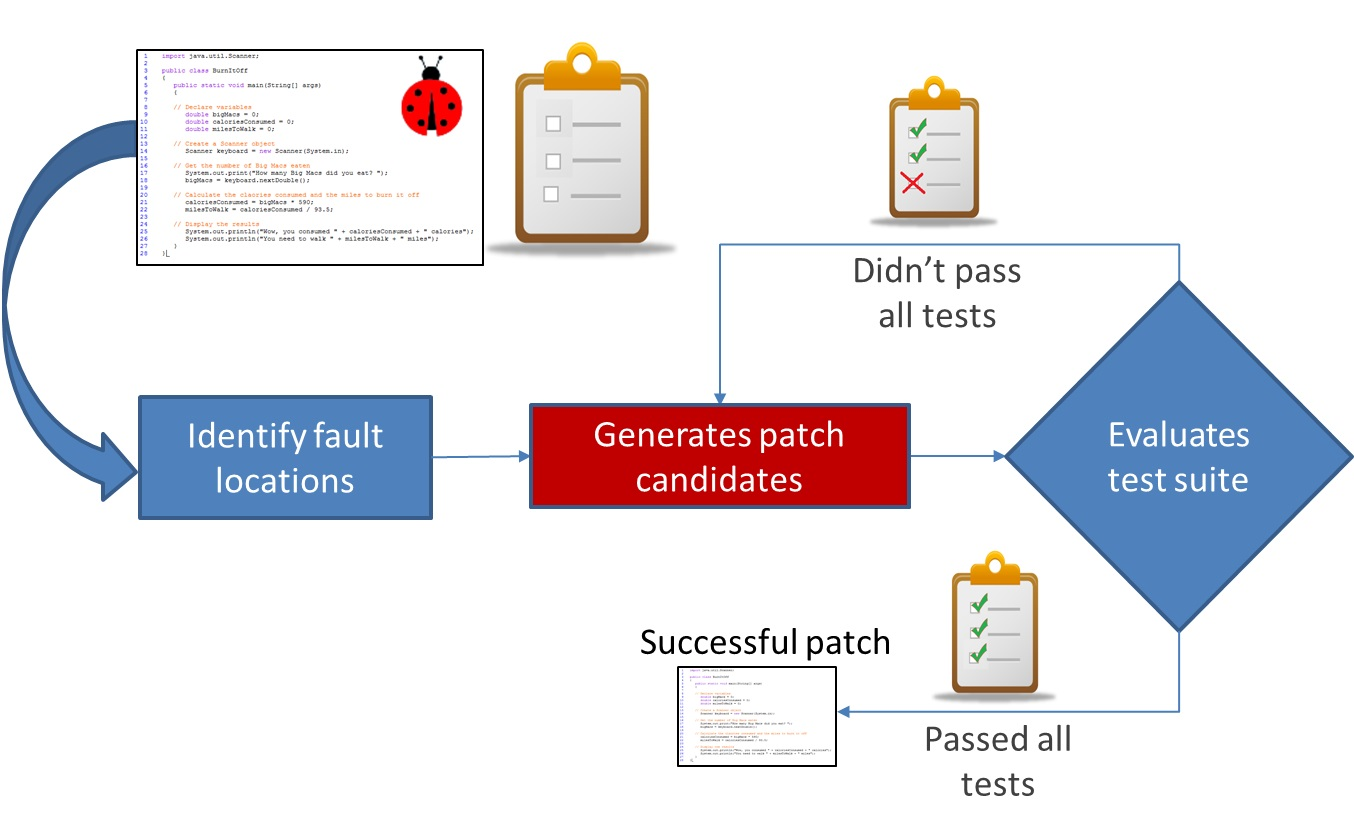
\includegraphics[scale=0.25]{Picture1}
  \caption{Generate and validate approach}
  \label{fig:generateandvalidate}
\end{figure}

The first step of this process is to localize the error in a particular 
statement. There is an extensive list of possible approaches in literature in 
order to perform this tasks~\cite{Jones05,Jones02,Chen02,legoues12,Qi13}, also there are several papers that have focused on the evaluation of the test suite~\cite{Qi13,fan15}; the main focus of this paper will be the step between these two, as highlighted in figure~\ref{fig:generateandvalidate} our main focus will be Generating patch candidates.

Once we know where the fault is located we proceed to create what we call 
``Candidate patches". Candidate patches are variations of the original program 
which may or may not be a patch for the bug(s) we are trying to fix. To 
create candidate patches we need to apply one or several mutation operators to 
the fault location. 

Once the tool has a set of candidate patches, it will run the test suite on each 
of those candidate patches. If it is able to find a candidate patch that can 
pass all the test cases in the test suite, that candidate patch will be 
considered a patch of the bug. If it is not able to pass all the test cases in 
the test suite, then it will go back to creating more candidate patches and will 
continue to do so until it reaches a stopping point, which may be a certain user 
defined number of generations or a user defined clock time limit.


In contrast to generate-and-validate there exist other techniques used for 
automatic program repair such as Synthesis-Based program 
repair~\cite{jin11,pei14} which uses constraints to build 
correct-by-construction patches via formal verification, inferred or 
programmer-provided contracts,
or specifications~\cite{smith15}. Also in contrast to search based approaches, there exist semantic based approaches such as SemFix~\cite{nguyen13}, DirectFix~\cite{mechtaev15} and SearchRepair~\cite{ke15} which use semantic analysis to create patches for buggy code.

Regarding generate-and-validate, in
order to select which mutation operator will be used, the 
first step is to define in what section of the code the fault is located. This can be determined in various ways, and 
there is 
a whole set of
possible approaches that can analyze this segment with different levels of certainty and 
requiring different characteristics from the source code and/or test 
suite~\cite{Jones05,Jones02,Chen02,legoues12,Qi13,Qi2013,Abreu07,wong09}. 

Regarding the association rule mining, to extract association rules from the data gathered in our study, we 
have transformed each of the mutation operator count and replacement count from 
each of the commits studied and created a transaction to be analyzed. A transaction in this context is a row of values that describes which mutation operators were applied in a single commit.

To use Apriori we need to further clarify basic concepts used by this approach: Confidence and Support.

Formally, we define Confidence as:

\begin{center}
$conf(X \implies Y) = \dfrac{supp(X \cup Y)}{supp(X)}$ 
\end{center}

Where X and Y are possible items in a transaction. In this context it is refering to mutation operators. As seen above Confidence is calculated according to its Support, where Support is an indication of how frequently the set of mutation operators (itemset) occurs in the transaction base.
Formally, we define Support as:

\begin{center}
$supp(X) = \dfrac{|\{t \in T; X \subseteq t\}|}{|T|}$
\end{center}

Where X is the itemset being analyzed and t is each individual transaction in the database of transactions T. 

\section{Generalization and Categorization of mutation operators} 
\label{categorization}

There are several possible mutation operators that can be applied to a location 
to modify the behavior of a program. To analyze the broad 
spectrum of mutation operators we categorized them into two groups: 
Statement-Edit and Template-Based. 

\subsection{Statement-Edit mutations}
There is a family of well-known approaches such as GenProg~\cite{legoues12}, 
TrpAutoRepair\cite{Qi13}, RSRepair~\cite{Qi14}, and AE~\cite{Weimer13} in which the main technique for 
creating candidate 
patches is by applying low level mutation operators (such as append, delete, or 
replace) which modify statements of source code to 
repair programs. A statement is the smallest standalone element that expresses 
some action to be carried out in a programming language. These tools are able to 
apply these mutation operators to statements in the source code to 
create candidate patches. These and several other techniques use randomized 
search for patch generation~\cite{arcuri08,bradbury10,Qi14,Weimer13}. 

\subsection{Template-based mutations}
Template-based mutation operators is the family of approaches that have 
predetermined templates to apply to specific sections of the code to 
modify the behavior of the program to make it possibly fix the error in the 
code being analyzed. In this family we have well known techniques such as PAR~\cite{kim2013}, 
SPR~\cite{fan15}, and 
Prophet~\cite{Long2016}.
 
PAR is the product of a study in which researchers examined a large number of 
human 
created patches and abstracted 10 different templates to be the most 
commonly used changes that human programmers perform to fix their 
code~\cite{kim2013}.
The 10 templates which they considered in their approach are the following:

\begin{tabular}{K{3.3cm}K{5cm}}
1) Null Checker & 6) Parameter Adder and Remover \\ 
2) Parameter Replacer & 7) Expression Adder and Remover \\  
3) Method Replacer & 8) Collection Size Checker \\
4) Expression Changer & 9) Range Checker\\
5) Object Initializer & 10) Class Cast Checker\\
\end{tabular}\\
 
In an effort to provide completeness, we also include 6 extra templates that are 
mentioned in the website of this 
approach\footnote{\url{https://sites.google.com/site/autofixhkust/home/fix-templates}} 
but aren't mentioned in the paper\cite{kim2013}. These extra templates provide new mutation operators that helps us compare and generalize to the other approaches: 

\begin{tabular}{K{3.3cm}K{5cm}}
1) Caster Mutator & 4) Lower Bound Setter  \\
2) Castee Mutator & 5) Upper Bound Setter  \\
3) Sequence Exchanger & 6) Off-by-one Mutator\\
\end{tabular}\\

Because of this, we consider a total of 16 PAR templates. There are other well known techniques in this domain, such as the SPR 
approach~\cite{fan15}, which is composed of a set of transformation schemas as 
follows:

\begin{tabular}{K{3.3cm}K{5cm}}
1) Copy and Replace & 4) Insert Initialization \\
2) Cond Refinement & 5) Cond Control Flow Introd  \\
3) Value Replacement  & 6) Condition Introduction 
\end{tabular}
\\

These transformation schemas can be seen as a generalization of some of the PAR 
templates, for example, ``Condition Introduction" can be seen as a superset of 
the corresponding templates in the PAR approach: Range Checker, Collection Size 
Checker, Class Cast Checker, and Null Checker. ``Condition Refinement" can be 
seen as a superset of 
Expression Adder and Remover. ``Insert Initialization" can be 
generalized from Object Initializer, Upper Bound Setter and Lower Bound Setter; ``Conditional Control Flow Introduction" can be 
seen as a subset of Sequence Exchanger;
``Value Replacement" can be seen as a superset of Method 
Replacer, Parameter Replacer, Castee Mutator and Expression Changer; and ``Copy 
and Replace" can be matched to Expression Adder. 

We also considered the program modification tool Kali~\cite{Qi15}, whose templates can be seen as subsets of some of the PAR templates or the extensions of the PAR templates mentioned above, for example Redirect Branch can be seen as a subset of ``Expression Changer", and Insert Return and Remove Statement are subsets of ``Expression Adder and Remover" accordingly. In the same way, we find similar mutation operators that can be seen as subsets of the extensions of the Par templates in studies such as~\cite{Offutt96,Offutt06}.

There is enough similarity between these approaches that they can be grouped 
into one category. We have chosen the PAR templates to represent this category 
since these templates provide a more concrete description of how the code is 
being changed, in order for us to replicate it; also, as mentioned before, all the SPR, Prophet and Kali templates are represented by one or several of the PAR templates, but not viceversa; and also the PAR templates represent templates specifically for the Java language, which is a common ground for the rest of the 
approaches considered and the benchmarks to evaluate the approach on.


\section{Building the model} \label{buildingTheModel}
In this section we describe the process we followed to build the probabilistic model mined from the most popular Java projects in Github which will be later evaluated.
\subsection{Selecting the corpus}
We started this process by cloning the 500 Java projects in Github 
with the most stars (collected in August 2016). When users star a project they are creating a bookmark for 
easier access, and showing appreciation to the repository maintainer for their 
work. Projects with more stars are more popular among the developers of Github 
and therefore more likely to be reviewed by other developers and have higher 
standards of code quality than projects with less stars. The methodology of 
gathering large,
popular, and active open source Java software repositories has been performed 
regularly for the analysis of empirical data by similar projects (eg,~\cite{Ray14}). 

We compiled the most recent 100 bug fixing commits per each project. Being able to tell apart a bug fixing commit from a non bug fixing commit is a difficult problem in repository mining~\cite{Bird09}. We filter these by applying a regular expression to the commit message in each of the commits in each of the projects that looks for words such as "fix", "bug", "issue", "problem", etc. following the guidelines by \cite{schroter06,Cubranic05,Fischer03}.
%\\
%\\
%$[Ff]ix(ed|es|ing)?(\backslash s)*([Bb]ug|[Ii]ssue|[Pp]roblem)?(s)?$
%\\
%\\
The intuition behind the regular expression approach is to filter commits where their 
commit message includes phrases such as: ``Fixed issue with variable x", ``Fix for 
problem discussed in meeting", ``I just fixed the script", etc.

We also added two extra filters to our search: First we had commits that only 
modify java source code. This is with the intention of looking only into bug 
fixing commits that fix java source code. Developers may also fix bugs in other 
sections of their projects, for example they may fix bugs in bash files, or xml 
code or any other kind of bug, and this wouldn't be relevant to our purpose of 
building a model that looks into the ways in which human developers fix their 
java code.

The last filter we applied to our search is to look only for the fixing commits 
that modify a maximum of 3 files per commit. This is for two reasons: first, we 
want to filter out big merges of code such as pull requests or initial commits 
where the commit is doing much more than just fixing a bug, which are the cases 
that we are interested in; and second, because earlier studies show that the larger the commit, the more probability it has of having tangled unrelated changes~\cite{Dias15,Herzig13,Matsuda15,Kawrykow11}, therefore these approaches usually work 
better when the fault is localized in a small number of locations.

\subsection{Identifying mutation operators from the developer's commits}

For each of these bug fixing commits, we then checked the version of the code 
before the fix was performed and after the fix was performed. We refer to these 
versions as the ``before-fix" version and the ``after-fix" version.

Next step is to know what changes are being performed from the before-fix version to 
the after-fix version, and we need to be able to analyze how often these changes match the mutation operators we are analyzing to understand what are 
the probabilities of each of them happening.

To do this we used two different widely used tools for mapping changes 
between two versions of code: Gumtree~\cite{falleri14} and QACrashFix~\cite{gao15}.
These tools create an AST representation of the program files for both the 
before-fix and after-fix representations of the programs for each of the files 
of the commit, and then use a set of heuristics to match the before-fix version 
with the after-fix version. Once this is done, the program's output is a set of 
changes needed to be performed to get from version before-fix to version 
after-fix.

We then created a program that goes through the list of changes and matches the changes performed from the before-fix to the after-fix versions into the different mutation operators. For example, if we want to analyze the simplest case: Null Checker, we go through all the actions performed to go from the before-fix to the after-fix versions; in each of the actions we ask if the node being manipulated is an If statement, we then  ask if the action being performed is an Insertion of a node. After we know that it is an insertion of an If statement, we then ask if the first condition within the If statement is an InfixExpression. An InfixExpression as defined by the Eclipse JDT API specification has the following form:
\\
\\
$InfixExpression: \\
Expression~InfixOperator~Expression
$
\\
\\  
Afterwards, we ask if the Expression following the InfixOperator is a NullLiteral. Once we know all this information we know that a null checker template was applied to the code, since we know that the developer added an If statement, whose conditional is conformed by an Expression being compared to a NullLiteral, so we count it as an instance of this template.




%\begin{figure}[!]
%\begin{verbatim}
%var res = 0
%for (ac <- actions) {
%  if(nodeClassName(ac.getNode) 
%    == "IfStatement"){
%      if (actionName(ac) == "Insert"){
%        if((nodeClassName(ac
%          .getNode.getChildren.get(0)) 
%            == "InfixExpression") && 
%              (nodeClassName(ac
%                .getNode.getChildren
%                  .get(0).getChildren.get(1)) 
%                    == "NullLiteral")){
%                      res += 1
%      }
%    }
%  }
%}
%\end{verbatim}
%\caption{Example of heuristic to spot the template Add Null Checker}\label{fig:codeSnippet}
%\end{figure}



\subsection{Two level probabilistic model}

We created two levels in the probabilistic model, the first one we will call the 
\textit{Mutation operator probabilistic model}, and the second level we will 
call the \textit{Replacements probabilistic model}.

The \textit{Mutation operator probabilistic model} is a probabilistic model that 
describes the probabilities to choose between the several different mutation 
operators in a particular fault location.

The \textit{Replacements probabilistic model} is the next level of the 
probabilistic model, which describes, if the ``Replacement" mutation operator is 
picked, what are the probabilities of replacing one statement for another. 

Once we created both models, we extended the tool GenProg4Java\footnote{https://bitbucket.org/clegoues/genprog4java}
 by implementing all the mutation operators mentioned in Section~\ref{categorization} and created a configuration in which the tool will select among the mutation operators according to the probabilities described by a given model. Next, a more fined grained explanation of both models:

\begin{figure}[!h]
  \centering
    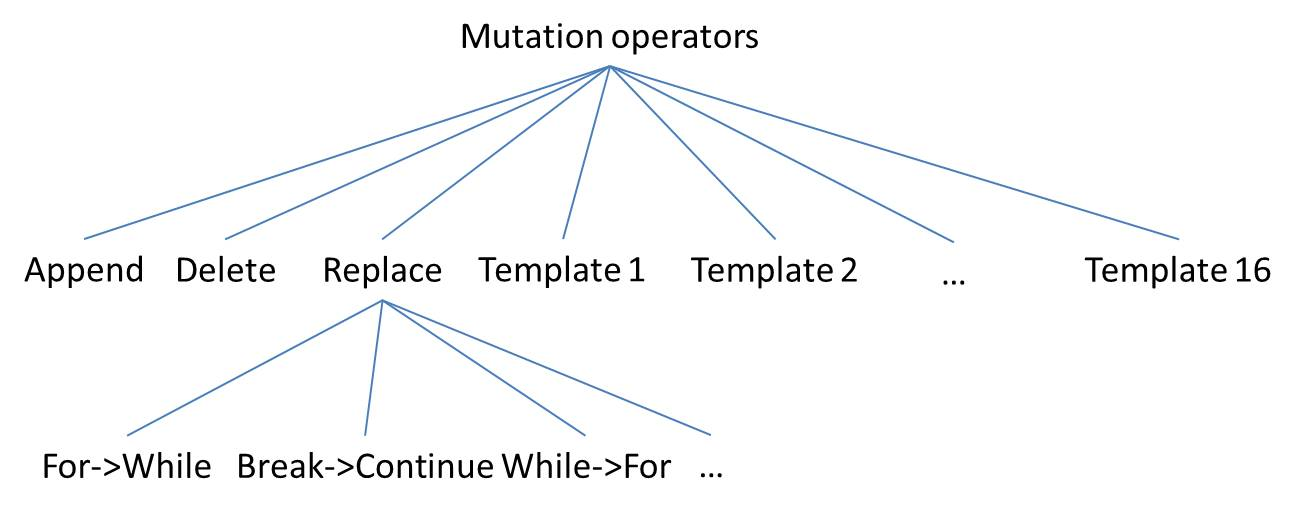
\includegraphics[scale=0.4]{Picture2}
  \caption{Two level probabilistic model}
  \label{fig:probModel}
\end{figure}

\subsubsection{Mutation operator probabilistic model}
To build the \textit{Mutation operator probabilistic model} we created 
a program that goes through these 
changes and matches these changes with the mutation operators we described 
earlier.

We sum the instances of each of the appearances of the mutation operators in the 
lists of changes created out of the differences between the before-fix and 
after-fix versions of each of the files in the 100 last bug fixing commits per 
each of the 500 projects; and these instance sums are the data we take to create 
our probabilistic model.

\subsubsection{Replacements probabilistic model}
To build the \textit{Replacements probabilistic model} we created a 
program similar to the one mentioned before\footnote{https://goo.gl/mMFbnQ
%REPLACE FOR CAMERA READY: https://github.com/mausotog/ReplacementsEmpiricalStudy
Note to reviewer: This link has been aliased for the purposes of the double 
blind review, the content is available, but the reviewer should notice that 
following the link mentioned before will potentially show the identity of the authors} that 
goes through these 
changes and when it encounters a  replacement mutation operator, then it looks 
at what kind of statement is being 
replaced and what kind of statement is replacing the other. We call these 
statements ``replacee" and ``replacer" accordingly.


We analyzed the 22 different kinds of statement detailed by Eclipse JDT as direct known subclasses of the class "Statement", and the probability in which each of 
them replaces another. For example, what is the probability that a For loop 
would replace a While loop, or the probability that a Break statement would 
replace a Continue statement, etc. Since there are 22 statement types and each of these 22 may 
replace each of these 22 statement types, we then have 484 combinations of 
replacement combinations.\footnote{The 22 statement types mentioned above are the following: AssertStatement, Block, BreakStatement, ConstructorInvocation, ContinueStatement, DoStatement, EmptyStatement, EnhancedForStatement, ExpressionStatement, ForStatement, IfStatement, LabeledStatement, ReturnStatement, SuperConstructorInvocation, SwitchCase, SwitchStatement, SynchronizedStatement, ThrowStatement, TryStatement, TypeDeclarationStatement, VariableDeclarationStatement, WhileStatement.\label{stmtNames}}

It is also worth noticing that these probabilities are not reciprocal, meaning 
that the probability of a For loop replacing a While loop is different from the 
probability of a While loop replacing a For loop, and the same applies to all 
the different statement types.

\section{Multiple edit association rule mining} \label{multEdit}

Edits that apply a single mutation (also known as "Single-edit" source code 
changes) as the ones studied so far in this study, are historically the most 
common subject of analysis in bug fixing tools and have been by far the most 
studied edits in the state of the art approaches 
\cite{Qi15,fan15,kim2013,Long2016,legoues12,Qi13,Qi14,xuan16}.
In these studies, most of the changes performed that result in 
successful patches are single edit changes, and this is ok for a initial stage 
of automatic program repair approach. This covers basic patches that humans 
perform, but the truth is that most bug fixes that humans perform in real 
software systems are much more complex and go a lot deeper than a single edit 
change. 

This study has gone one step further and gives a initial analysis of multi edit 
source code changes by extracting association rules between single edit changes 
to create chains of single edit changes the way humans create them.

We use the 
well known association rule mining algorithm
Apriori~\cite{Agrawal94,Liu98,Zaki2000} in which we identify the frequent 
individual items in the set of transactions (commits in this context) and then we extend these sets into 
larger sets as long as those item sets appear sufficiently often in the database 
of transactions, which in our case would be the database of transactions created 
by each of the commits studied.

We have divided our association rule mining into the two different models as 
follows:


\subsection{Mutation operator and replacement rules}

To create these association rules among several mutation operators, we mine the transactions made out of the commits created by humans in the corpus of projects studied and we look for rules that have at least 90\% Confidence, where Confidence is an indication of how often the rule has been found to be true. 

These rules are ranked by their confidence; in this case, the top 5 rules shown below have a confidence of a 100\% which means that in 100\% of the cases studied, every transaction that showed the antecedent also shows the consequent; and they are obtained with a 1\% support, which means that each of these rules individually show in at least a 1\% of all the transactions of the overall corpus. We show the 5  top association rules found for the mining of single edit mutation operators.


%Minimum support: 0 (1 instances)
%Minimum metric <confidence>: 0.9
%Number of cycles performed: 20
\begin{itemize}
\item Replace \& Delete $\implies$ Append
\item Delete \& AddNullCheck $\implies$ Append
\item Replace \& SeqExchanger $\implies$ Append
\item Replace \& ParamReplacer $\implies$ Append
\item Delete \& CasteeMutator $\implies$ Append
%\item Replace \& Delete \& ParamReplacer $\implies$ Append
%\item Replace \& AddNullCheck $\implies$ Append
%\item Replace \& Delete \& SeqExchanger $\implies$ Append
%\item Delete \& ExpressionAdder $\implies$ Append
%\item Delete \& AddNullCheck \& ParamReplacer $\implies$ Append
\end{itemize}

Append is the most common single edit mutation operator. This behavior is reflected in the fact that it is the most common consequent being the consequent in 5 out of 5 of the top 5 association rules. The authors are showing the top 5 association rules to give an example of what the rules look like. If the reader would like to know the full list of association rules mined in this study, the authors have made available the full list with over 12.000 rules with over 90\% Confidence and 0.01\% Support.\footnote{https://goo.gl/UT8QbI}
%REPLACE FOR CAMERA READY: https://github.com/mausotog/ReplacementsEmpiricalStudy/blob/master/ResultsAssociationRuleMiningMutOperators.txt

Similar to the case detailed before, we have analyzed the association rules for the replacements model. We obtained the following rules with a 0.01\% Support and 90\% Confidence.
10 Best rules found:
%Minimum support: 0.0001 (1 instances)
%Minimum metric <confidence>: 0.9
%Number of cycles performed: 20
\begin{itemize}
\item Block replaces ReturnStatement \& ExpressionStatement replaces IfStatement $\implies$ Block replaces IfStatement
\item VariableDeclarationStatement replaces AssertStatement $\implies$ SwitchCase replaces BreakStatement
\item EnhancedForStatement replaces TryStatement $\implies$ ExpressionStatement replaces ReturnStatement
\item ForStatement replaces TryStatement $\implies$ ExpressionStatement replaces VariableDeclarationStatement
\item VariableDeclarationStatement replaces EnhancedForStatement $\implies$ ExpressionStatement replaces VariableDeclarationStatement
\item VariableDeclarationStatement replaces ForStatement $\implies$ ExpressionStatement replaces VariableDeclarationStatement
\item ForStatement replaces TryStatement $\implies$ IfStatement replaces TryStatement
\item VariableDeclarationStatement replaces ForStatement $\implies$ ForStatement replaces TryStatement
\item ForStatement replaces TryStatement $\implies$ VariableDeclarationStatement replaces ForStatement
\item VariableDeclarationStatement replaces ForStatement $\implies$ IfStatement replaces TryStatement
\end{itemize}

Similar to the one described above, the authors have made available the full list of association rules with over 90\% Confidence and 0.01\% Support.\footnote{https://goo.gl/omk60t}
%REPLACE FOR CAMERA READY: https://github.com/mausotog/ReplacementsEmpiricalStudy/blob/master/ResultsAssociationRuleMiningReplacements.txt



%\subsection{10 fold cross validation}




\section{Evaluation} \label{evaluation}
Building the model and evaluating it is a time consuming process. Therefore, the first step in our effort to know if the probabilistic model is a promising idea, is to perform an evaluation on a subsection of the model. We performed two different evaluations on a subsection of the model, and finally we performed a larger evaluation with the complete model. The first of these evaluations is a 10 fold cross 
validation of the model; the second, a run on a case study to check how 
much faster we can find a patch with the probabilistic model vs the equally 
distributed approach; and finally an evaluation on fifteen independent real life bugs.

\subsection{Evaluating how the model will generalize to an independent data set}

%Our initial sanity check was performed on the replacements model. At this point, 
We segregated the projects into 10 
different folds assigned at random. For each of the 
folds we would take 1 fold for testing and the remaining 9 folds for training. 
Afterwards we analyze how often do the training data is able to predict the 
testing data. This is performed 10 times, one time per each fold and then it is 
averaged to see how commonly is the training data able to predict the testing 
data.

In this initial sanity check we are comparing two distributions: the sub-model 
that is built from the remaining 9 folds, and the distribution of the testing 
data. We need to analyze how often one of the distributions (the sub-model 
training data) predicts the other distribution (the distribution of the fold we 
are trying to predict). 

Since the main focus of this step is to check whether the behavior of the 
current approaches would perform faster with the probabilistic model as opposed 
to the current equally distributed scheme; we rank the first five choices each 
of the models would take and see how many of the instances in the testing data 
match those first five guesses. Five guesses is the point of inflection where the maximum difference between the two approaches happen. After five guesses, the slope starts to flatten, which is why we picked five guesses as our comparison point.

\begin{table}[ht]
\begin{tabular}{llllllllllllllllllllll}
\hline
As & Bl & Br & Cl & Co & Do & Em & EF & Ex & Fo & If \\
0\%&2\%&0\%&2\%&5\%&0\%&0\%&0\%&43\%&0\%&22\% \\
\hline 
La & Re & SC & Ca & Sw & Sy & Th & Tr & TD & VD & Wh \\
0\%&0\%&2\%&2\%&0\%&0\%&3\%&2\%&0\%&19\%&0\% \\
\hline
\end{tabular}
\\
\caption{Example of the Return Statement row of a sub-model created from 
the training data. Replacee probabillities of the replacer ReturnStatement. The acronyms represent the statement kinds detailed in footnote \ref{stmtNames}}
 \label{fig:exPredReturn} 
\end{table} 

%\begin{figure}[!h]
%  \centering
%    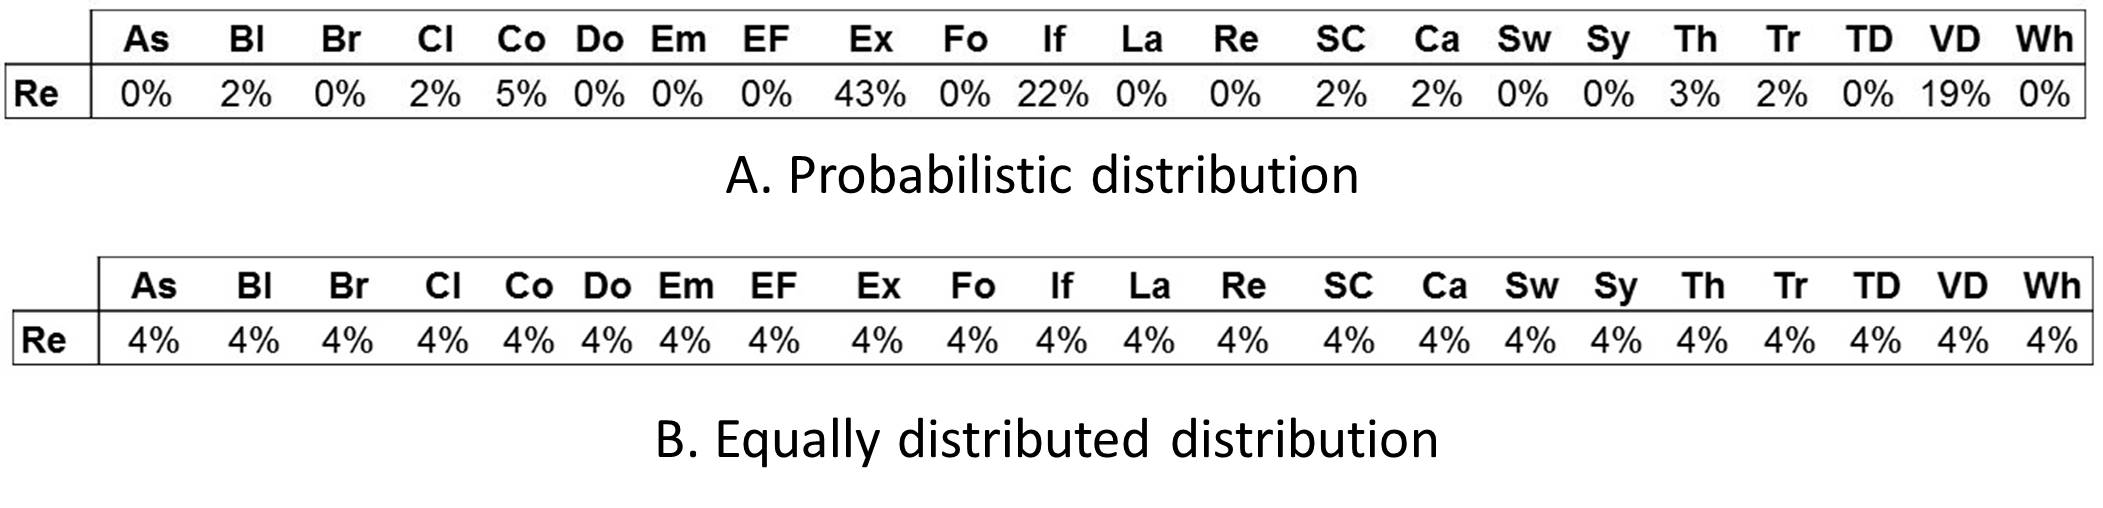
\includegraphics[scale=0.25]{sanity5}
%  \caption{A)  B) Example of return statement with equally distributed 
%probability. }
% 
%\end{figure}

To illustrate the point, consider a simple example. Assume we have a 
distribution in fold 1 that describes how many times each statement is replaced 
by other kinds of statements in this fold 
only, this is what we denominate testing data and we represent it with $E_{n,m}$ 
where $n$ is the statement being replaced (replacee) and $m$ the statement it is 
replaced by (replacer); likewise we have a probabilistic sub-model created from 
folds 2-10 inclusive $TP_{n,m}$ where $\forall n,m: 1<=n<=22 \land 1<=m<=22$, 
that describes how often each statement is replaced by 
other kinds of statements, this is what we call the training data. 

In 
particular, assume we are analyzing the Return statement (Row 13). We want to 
predict 
how well the sub-model created from folds 2-10 is able to predict the testing 
data; in this particular case, how well is the section of the sub-model that 
describes the Return Statement able to predict the instance count of the 
statements that replace a Return Statement in the testing data.

Assume the training data is a sub-model $TP_{n,m}$ which contains a row 
$TP_{13,m}$ as the one shown in figure~\ref{fig:exPredReturn}A, and the testing data is a distribution that describes 
how many instances of returns were replaced by different statements.
%as follows: 
%A return statement was replaced by a Expression Statement 4 times $E_{13,9} = 
%4$; by an If 
%Statement 2 times $E_{13,11} = 2$; by a Continue Statement 2 times $E_{13,5} = 
%2$; by a Do Statement 1 time $E_{13,6} = 1$;
%and by a Try Statement 1 time $E_{13,19} = 1$. As a clarification, this is a 
%fictional example 
%to explain how the prediction is being analyzed.
For each of the statements we would take the top five guesses from each row in 
the sub-model and count the percentage of instances of the testing data that were correctly 
predicted by the sub model. 

In this example, the top five guesses in this row would be: The most 
likely statement chosen to replace a Return Statement according to this row in 
this fictional sub-model would be a Expression Statement (Ex) $TP_{13,9} = 43\%$ 
which means that there is a 43\% of probability to replace a Return Statement. 
The second and following most likely would be an If Statement (If) $TP_{13,11} = 22\%$, Variable Declaration (VD)  $TP_{13,21} = 19\%$, 
Continue Statement (Co)  $TP_{13,5} = 5\%$, and Throw Statement (Th) $TP_{13,18} = 3\%$. We then compare how many instances of the testing data were correctly predicted 
by these top five guesses of this row in the sub-model. 
%In this example, we will 
%look at the instances that match the top five guesses in the testing data, which 
%would be: Expression Statement $E_{13,9} = 4$, If Statement $E_{13,11} = 2$, and 
%Continue Statement $E_{13,5} = 2$. Since Do 
%Statement $E_{13,6} = 1$ and Try Statement $E_{13,19} = 1$ were not within the 
%top five guesses, then the 
%instances in these two categories won't be considered a successful match, but 
%the former three would. 

%Based on this information, we can say that the 4 instances of Expression 
%Statement replacing a Return Statement in the testing data were correctly 
%predicted by the sub-model; the same with the 2 instances of the If Statement 
%and the 2 instances of the Continue Statement. The instance of the Do Statement, 
%and the instance of the Try Statement, would be considered as not correctly 
%predicted by the sub-model. In this case, since the sub-model correctly 
%predicted 8 out of 10 instances, we say that the sub-model correctly predicted 
%80\% of the instances in the testing data. 

To contrast this with the equally distributed approach used currently, 
we assign all the statements, the same probability of being chosen to replace 
the statement being analyzed. We denominate the equally distributed approach 
$TE_{n,m}$ where $\forall n,m: 1<=n<=22 \land 1<=m<=22 \land TE_{n,m} = 4.54\%$. 
We have been analyzing the Return Statement in this particular example, as 
detailed in figure~\ref{fig:exPredReturn}B. To get the top five choices of the 
equally distributed schema we just pick five choices at random, since all of 
them have the same probability, which is how the current approach handles what 
statement to pick.

%For example, if the approach picks at random the statements: Assert Statement 
%$TE_{13,1}$, 
%Do Statement $TE_{13,6}$, Expression Statement $TE_{13,9}$, Throw Statement 
%$TE_{13,18}$ and Try Statement $TE_{13,19}$. Then we 
%would match how many of the instances in the testing data were correctly 
%predicted by this equally distributed schema.

%In this example, the 4 instances of Expression Statement $E_{13,9} = 4$, the 
%instance of Do 
%Statement  $E_{13,6} = 1$, and the instance of Try Statement $E_{13,19} = 1$ 
%would be considered to be correctly 
%predicted; while the 2 instances of If Statement $E_{13,11} = 2$, and the 2 
%instances of 
%Continue Statement $E_{13,5} = 2$ would be considered to be incorrectly 
%predicted. Since the 
%equally distributed approach in this example correctly guessed 6 out of 10 
%instances of the testing data, we would then say that in this particular case, 
%the equally distributed approach correctly predicted 60\% of the instances in 
%the testing set.  

\begin{figure}[!h]
  \centering
    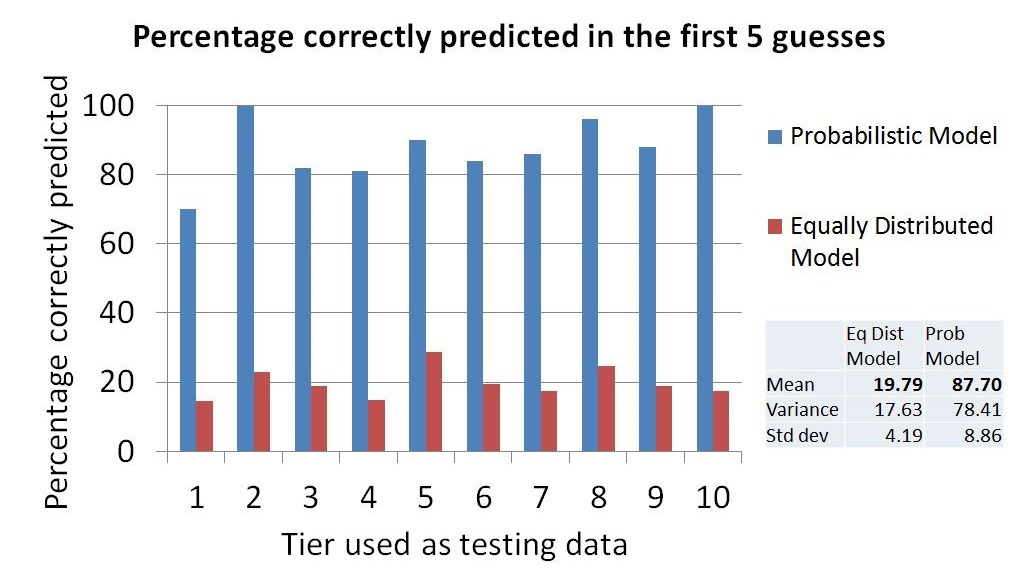
\includegraphics[scale=0.33]{sanity1}
  \caption{Correctly predicted percentage by applying 10 fold cross validation}
  \label{fig:results10fcv}
\end{figure}

We ran this experiment with all the rows $n$ in the sub-model $TE_{n,m}$ and 
$TP_{n,m}$ for each of the 10 
folds. The results are detailed in figure~\ref{fig:results10fcv}. As we can see 
in this graph, the red bars represent the results of the percentage of correctly 
predicted instances of the testing data in each particular fold by the top five guesses of the equally distributed approach; while the blue 
bars represent the percentage of correctly predicted instances using the top five 
guesses of the sub-model of each of the folds. We have a mean of 19.79\% 
correctly predicted instances through the different folds when using the equally 
distributed schema, while we get a mean of 87.70\% correctly predicted instances 
through the different folds when using the probabilistic model. 

\subsection{Case study}
After performing the 10 fold cross validation, we know that the model built by 
gathering cases mined from Github predicts with very high accuracy all the 
subsets of the data gathered, which implies that the data is consistent among 
the folds and outperforms the current equally distributed model in every case. 

The natural next step would be to try the model with an example taken from 
outside of the collected cases from Github. Therefore we evaluated our model 
with an example of a basic bug in a method as shown in figure~\ref{fig:initialExample}. The purpose of this method is to calculate the median 
of three numbers, and there is a bug as indicated by the highlighted text where 
instead of $ret = z;$ it should be $ret = x;$ to have a correct output 
for all cases.

\lstdefinestyle{base}{
  language=Java,
  emptylines=1,
  breaklines=true,
  basicstyle=\ttfamily\color{black},
  moredelim=**[is][\color{red}]{@}{@},
  xleftmargin=20pt, frame=bt, basicstyle={\small\tt}, numbers=left, keywordstyle=\bfseries, 
	numberstyle=\scriptsize\tt,  moredelim=[is][\color{red}]{@}{@}, deletekeywords={}, captionpos=b, belowskip=1pt, autogobble=true
}

\begin{figure}[t]
\begin{lstlisting}[frame=single,style=base]
  public int mid(int x, int y, int z){
    int ret = z;  
    if(y<z){
      if(x<y){
        ret = y;
      }else if(x<z){
        ret = z; @//bug, it should be ret=x;@
      }
    }else{
      if(x>y){
        ret = y;
      }else if(x>z){
        ret = x;
      }
    }
    return ret;
  }	
	\end{lstlisting}
	\caption{Source code of an independent example. Bug to be fixed is annotated and highlighted}
	\label{fig:initialExample}
\end{figure}



%\begin{figure}[!h]
%  \centering
%    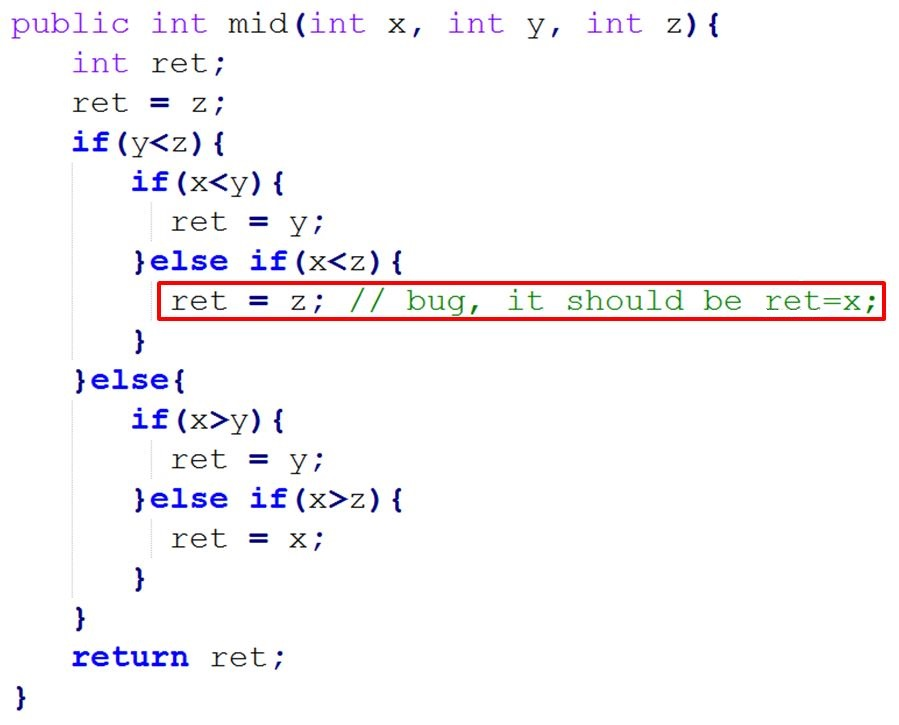
\includegraphics[scale=0.35]{sanity2}
%  \caption{Source code of an independent example. Bug to be fixed is annotated %and highlighted}
%  \label{fig:initialExample}
%\end{figure}

To be able to do this, we restructured the code of the tool ``GenProg4Java",\footnote{https://bitbucket.org/clegoues/genprog4java/} which is the Java version of the 
well known tool Genprog~\cite{legoues12}. This tool provides the work-flow 
for many generate-and-validate approaches to be implemented. We restructured the 
tool to be able to select the mutation operators between a 
probabilistic model, and the default (equally distributed).

We then ran the tool on the code in figure~\ref{fig:initialExample} using both 
the probabilistic model and the equally distributed model. Since this is a 
case study for sanity checking, we start by evaluating it on a subset of 
the mutation operators. We first evaluate it in two different sets: 1) Only using the $Replace$ mutation operator, and 2) Using only $Append,~
Remove~and~Replace$ mutation operators. The results are detailed in figures 
\ref{fig:resultsReplace} and \ref{fig:resultsARR}. 

Generate-and-validate, as explained before, works by creating variants of the 
source code by applying mutation operators to the original source code. 
Therefore, a large number of variants created before finding a patch means that 
it takes longer to find a patch, than a small number of variants. We can imply by this 
that in these graphs, the smaller number of variants in each case, means that 
the patch was found faster, than with a larger number of variants. It is also 
noticeable that this tool uses genetic programming in its workflow, therefore we 
run the tool with 10 different seeds to be able to abstract the results 
and not focus on a particular seed.

In figure~\ref{fig:resultsReplace} we consider only the mutation operator 
$Replace$, which means that the tool will disregard all other mutation 
operators and will only apply Replace operations using the probabilistic model 
of Replacements. This is because at this step we are evaluating our model in a 
subset of the mutation operators to understand if it makes sense to move forward and 
continue implementing the rest of the mutation operators.

In this graph we can analyze the runs with 10 different seeds, contrasting the 
number of variants it takes to find a patch using the probabilistic approach 
(blue bar), with the number of variants it takes to find a patch using the 
equally distributed approach (green bar). 

As we can derive from the graph, the probabilistic approach was able to find a 
patch faster than the equally distributed for all the seeds tested. In some 
cases as seed 5, 7 and 10, the patch using the probabilistic approach was found 
in one of the first variants, therefore the number is so low that it doesn't 
show in the graph. In average, we found that by using the probabilistic model we 
could find a patch in 23.8 variants, while it took an average of 60.5 variants 
to find a patch using the equally distributed model.

\begin{table}[ht]
\begin{tabular}{lR{0.1cm}R{0.1cm}R{0.1cm}R{0.1cm}R{0.1cm}R{0.1cm}R{0.1cm}R{0.1cm}R{0.1cm}R{0.1cm}R{0.5cm}R{0.5cm}}
\hline
\textbf{Seed} & \textbf{0} & \textbf{1} & \textbf{2} & \textbf{3} & \textbf{4} & \textbf{5} & \textbf{6} & \textbf{7} & \textbf{8} & \textbf{9} & Avrg & StdDev  \\
\hline
\textbf{Prob} & 48 & 19 & 81 & 41 & 0 & 11 & 0 & 25 & 13 & 0 & 23.8 & 24.8 \\

\textbf{Eq Dist} & 49 & 34 & 89 & 98 & 4 & 11 & 80 & 25 & 13 & 202 & 60.5 & 57.1\\
\hline
\end{tabular}
%\\
%\\
%\center
%\begin{tabular}{|lrrr|}
%\hline
%& Average & Variance & Std Dev \\
%\hline
%\textbf{Prob Model} & 23.8 & 615.8 & 24.8\\
%
%\textbf{Eq Dist} & 60.5 & 3261.5 & 57.1\\
%\hline
%\end{tabular}
%\\
\center
  \caption{Number of variants it takes to find a patch (starting at 0) using replace to guide the search for a patch of the case study}
  \label{fig:resultsReplace}
\end{table} 

%\begin{figure}[!h]
%  \centering
%    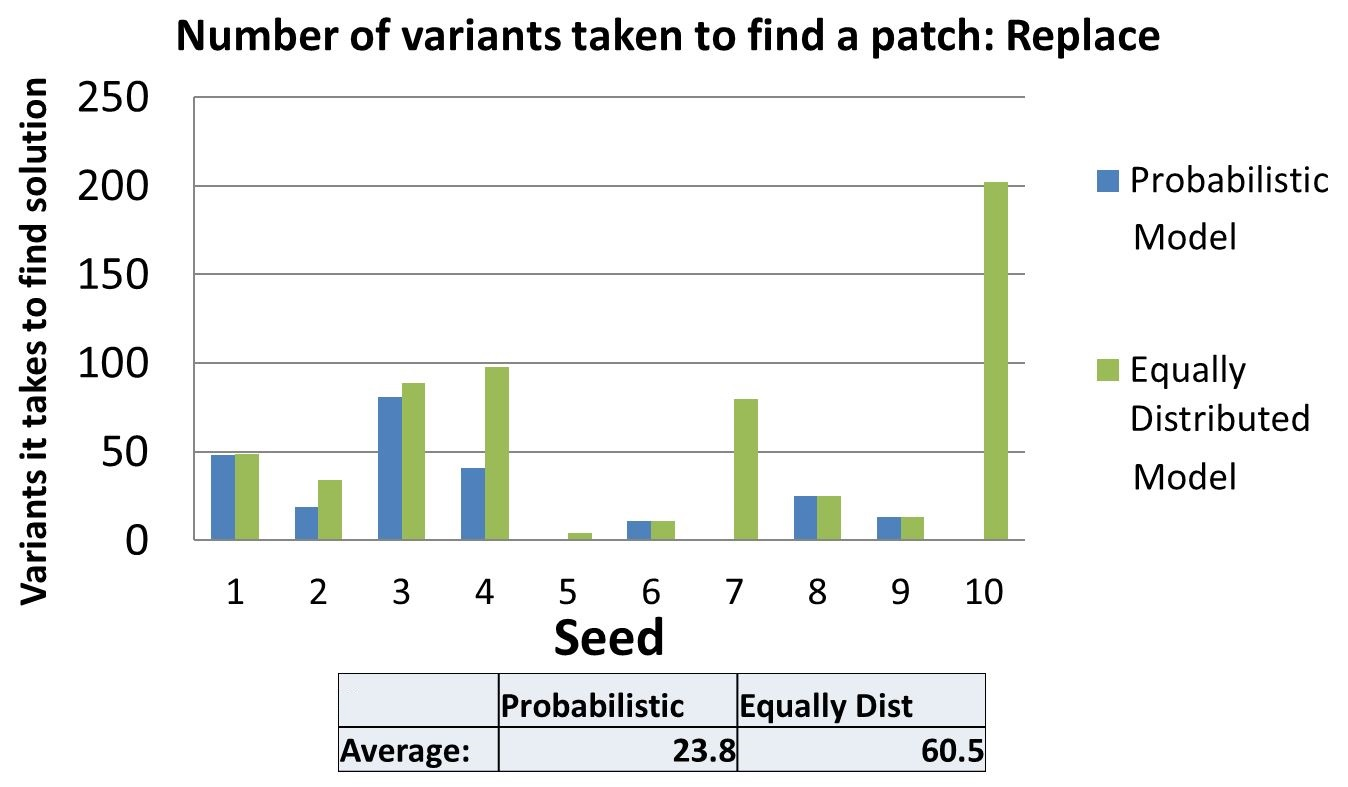
\includegraphics[scale=0.25]{sanity3}
%  \caption{Using replace to guide the search for a patch of the case study}
%  \label{fig:resultsReplace}
%\end{figure}

In figure~\ref{fig:resultsARR}, we consider three mutation operators: Append, 
Remove and Replace. In this case we can also notice that in seeds 7 and 10 the 
number of variants it takes to find a patch using the probabilistic model is 
close to 1 therefore it is hard to notice it in the graph. In this case the data 
shows that using the probabilistic model we obtain a mean of 22.6 variants 
before finding the patch, while it takes an average of 41.4 variants to find the 
patch using the equally distributed approach. We consider of importance to notice that in both experiments the probabilistic model outperformed the equally distributed model in every single case.


\begin{table}[ht]
\begin{tabular}{lR{0.1cm}R{0.1cm}R{0.1cm}R{0.1cm}R{0.1cm}R{0.1cm}R{0.1cm}R{0.1cm}R{0.1cm}R{0.1cm}R{0.5cm}R{0.5cm}}
\hline
\textbf{Seed} & \textbf{0} & \textbf{1} & \textbf{2} & \textbf{3} & \textbf{4} & \textbf{5} & \textbf{6} & \textbf{7} & \textbf{8} & \textbf{9}  & Avrg & StdDev  \\
\hline
\textbf{Prob Model} & 8 & 20 & 23 & 42 & 4 & 11 & 0 & 29 & 80 & 0  & 22.6 & 23.7\\

\textbf{Eq Dist} & 8 & 66 & 23 & 42 & 4 & 11 & 2 & 38 & 81 & 139 & 1704.0 & 41.3 \\
\hline
\end{tabular}
\\
\\
%\center
%\begin{tabular}{|lrrr|}
%\hline
%& Average & Variance & Std Dev \\
%\hline
%\textbf{Prob Model} & 22.6 & 563.0 & 23.7\\
%\textbf{Eq Dist} & 41.4 & 1704.0 & 41.3\\
%\hline
%\end{tabular}
%\\
%\center
  \caption{Number of variants it takes to find a patch (starting at 0) using append, remove and replace to guide the search for a patch of 
the case study}
  \label{fig:resultsARR}
\end{table} 
%\begin{figure}[!h]
%  \centering
%    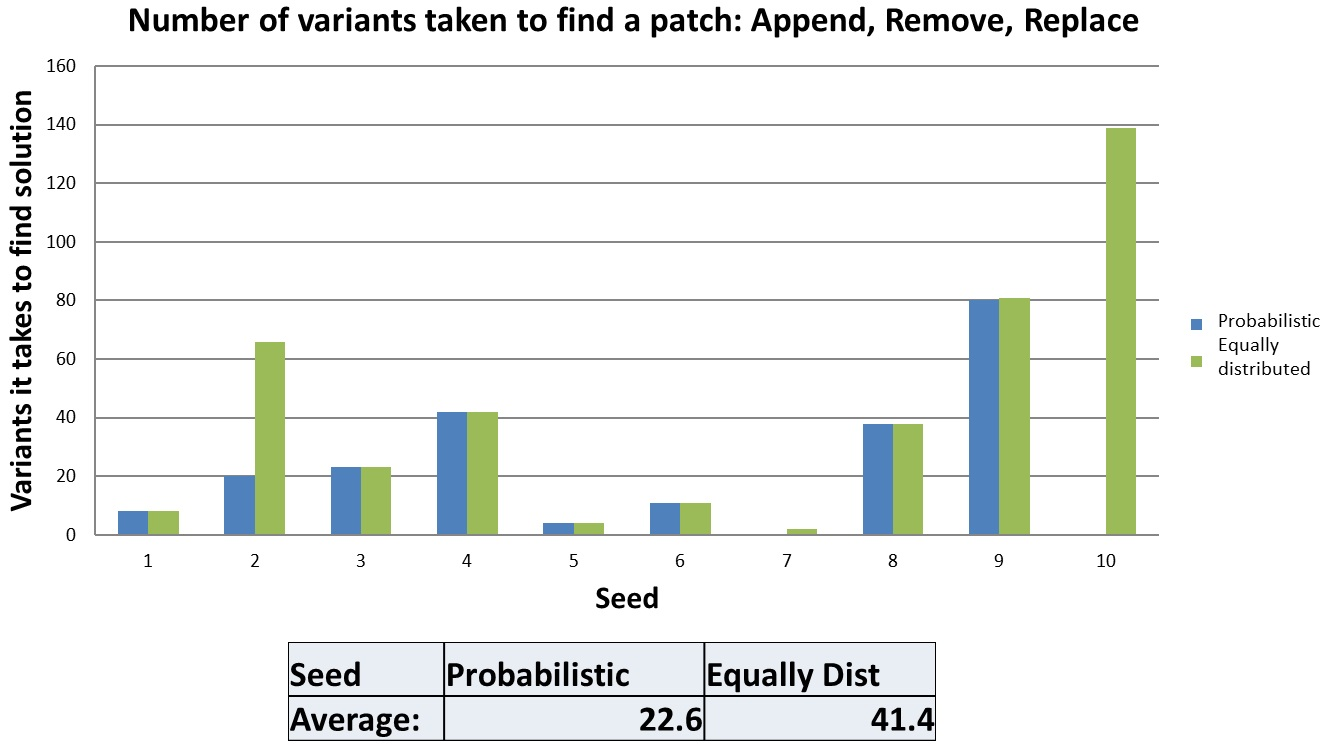
\includegraphics[scale=0.25]{sanity4}
%  \caption{Using append, remove and replace to guide the search for a patch of 
%the case study}
%  \label{fig:resultsARR}
%\end{figure}

\subsection{Single line bugs with Human Injected Fault Localization}
After having very successful results in the first two evaluations with a subset of the model, we decided 
to increase our data by building the whole model with 500 projects in Github with more 
stars. This is to generate the largest code base so far to the best 
of our knowledge, surpassing all the previous state of the 
art~\cite{long15,Soto15,zhong15,matias15,xuan16}. 

At this point, by analyzing our dataset, 
we found that the Template-Based mutations comprise 29.26\% of the corpus of 
instances found, while Statement-Edit mutations make up 70.74\% of the 
corpus. Since this idea seems promising at this point we decided to implement the rest 
of the mutation operators. We implemented these 16 templates in GenProg4J, and generated the functionality 
to be able to select which subset of mutation operators to apply in a particular 
run.

We are interested in evaluating our new approach with real life bugs taken from 
open source projects that have a long history of maintainability and 
scalability. For these reasons, we chose Defects4j~\cite{just14} as our 
evaluation platform. Defects4j is a database and extensible 
framework providing real bugs to enable reproducible studies in software testing 
research~\cite{just14}. This database of bugs contains 357 real bugs from 5 
real-world open source programs, and each of these cases is accompanied by a 
comprehensive test suite with test cases that expose the bug. This database also provides 
the corresponding human-generated patch, which is the version of the code written by a human 
developer to patch the bug. Due to these features Defects4j has previously been 
subject for evaluation of important APR approaches~\cite{Durieux15}.

To perform our evalutation, we ran our approach in a physical server that 
consists of 16 processors Intel(R) Xeon(R) CPU E5-2699 v3, with 2.30 GHz each 
processor, 46080 KB cache each, and 32 GB RAM memory, operating system Ubuntu 
14.04.5 LTS. We set the size for each population to 40 for consistency with 
previous work~\cite{legoues12,kim2013} and a timeout of 4 hours since there is 
the need of several generations of mutant creations needed to assess the 
performance of this approach~\cite{arcuri11}.

For this evaluation we tested the mutation operators using three different sets 
of operations: 1) Statement-Edit mutations only 2) Template-based mutations 
only 3) All mutations.

Since historically automatic program repair has worked better with single line 
patches, we decided to first test bugs that required a single line edit to get 
patched. We analyzed the first 3 bugs from each of the projects that required a 
single line edit.\footnote{The bugs that met this criteria are the following: Chart 1, 
Chart 8, Chart 20, Closure 10, Closure 14, Closure 18, Lang 6, Lang 16, Lang 21, 
Math 2, Math 5, Math 10, Time 4, Time 16 and Time 19.}

Several evaluations in the past use an off-the-shelf fault localization technique when evaluating a new way to navigate the search space, which introduces a lot of noise and randomness to the result of the patch creation and selection process. To diminish the degree of randomness in this experiment, we will be using Human Injected Fault Localization, a technique in which the researcher indicates to the APR approach the section of the code that contains the defect. In these cases we picked the faulty statements to be the statements which the human developers modified to patch the code.

From these 15 bugs we were able to find patches for 5 of them as described in table \ref{tab:singleLineBugs}. It is also worth mentioning that the numbers shown in the table are the mean from the solutions found running the tool with 20 different seeds. 

In the first row of Table \ref{tab:singleLineBugs} (Closure \#10) we can see that in all three comparisons (Statement-Edit Only, Template-Based Only, and All mutations), the approach using the probabilisitc model performs better than its counterpart using the equally distributed model. This happens as well in all cases of bugs Math \#2 and Time \#19 except for the cases where no patch was found. Different from this, in bugs Chart \#1 and Closure \#18 the equally distributed approach finds a patch faster in average. This is due to the fact that removal mutations such as Deletion and Expression Changer are more likely to be picked by the equally distributed model than the probabilistic model since developers use these editions less often than others. But these editions have been seen in the past to make the test cases pass even if the edition did not fixed the bug as per the opinion of developers as indicated in~\cite{kim2013}.

Our results also show that applying mutation operators from both categories together, benefits the process by finding the patch faster, than when restricting the mutation operator pool to just one of the categories. For the Statement-Edit category: 3 out of 6 were fixed faster when combining it with Template-Based mutations, and 3 out of 6 were slower. For the Template-Based category: 4 out of 8 were fixed faster when combining it with Statemtent-Edit mutations, 2 out of 8 were the same, and 2 out of 8 were slower.

\begin{table*}\centering
\ra{1.3}
	\resizebox{\textwidth}{!}{
\begin{tabular}{|r|rr|rr|rr|rr|rr|rr|}
\hline
  &\multicolumn{4}{c|}{\textbf{Stmt-Edition}} & \multicolumn{4}{c|}{\textbf{Temp-Based}} & \multicolumn{4}{c|}{\textbf{All mutations}} \\  
 \hline
 \textbf{Bug Name}  & \multicolumn{2}{c|}{\textbf{Equally Dist}} & \multicolumn{2}{c|}{\textbf{Probabilistic}} & \multicolumn{2}{c|}{\textbf{Equally Dist}} & \multicolumn{2}{c|}{\textbf{Probabilistic}} & \multicolumn{2}{c|}{\textbf{Equally Dist}} & 
\multicolumn{2}{c|}{\textbf{Probabilistic}} \\

 Closure \#10 & \color{OliveGreen}{221.0}& \color{blue}{100\%} & \color{OliveGreen}{179.5} &\color{blue}{100\%} & \color{OliveGreen}{175.1}&\color{blue}{100\%} & \color{OliveGreen}{121.3}&\color{blue}{100\%} & \color{OliveGreen}{163.3}&\color{blue}{100\%} & \color{OliveGreen}{157.4}&\color{blue}{100\%} \\

 Closure \#18 & \multicolumn{2}{c|}{Not found} & \multicolumn{2}{c|}{Not found} & \color{OliveGreen}{36.2}&\color{blue}{100\%} & \color{OliveGreen}{197.5}&\color{blue}{100\%} & \color{OliveGreen}{45.0}&\color{blue}{100\%} & \color{OliveGreen}{139.0}&\color{blue}{100\%} \\

 Math \#2 & \multicolumn{2}{c|}{Not found} & \multicolumn{2}{c|}{Not found} & \color{OliveGreen}{109.4}&\color{blue}{0\%} & \color{OliveGreen}{39.6}&\color{blue}{0\%} & \color{OliveGreen}{109.4}&\color{blue}{0\%} & \color{OliveGreen}{39.6}&\color{blue}{0\%} \\

 Time \#19 & \color{OliveGreen}{94.1}&\color{blue}{100\%} & \color{OliveGreen}{80.7}&\color{blue}{100\%} & \multicolumn{2}{c|}{Not found} & \multicolumn{2}{c|}{Not found} & \color{OliveGreen}{135.1}&\color{blue}{100\%} & \color{OliveGreen}{91.9}&\color{blue}{100\%} \\

 Chart \#1 & \color{OliveGreen}{1.8}&\color{blue}{0\%} & \color{OliveGreen}{7.3}&\color{blue}{0\%} & \color{OliveGreen}{4.9}&\color{blue}{0\%} & \color{OliveGreen}{19.0}&\color{blue}{0\%} & \color{OliveGreen}{2.2}&\color{blue}{0\%} & \color{OliveGreen}{4.8}&\color{blue}{0\%} \\

\hline
 
\end{tabular}
}
\ra{1.3}
		\caption{Value on the left of each slot (green): Number of variants taken to find a patch in single line bugs. Value on the right of each slot (blue): Percentage according to the number of patches that passed the second test suite}\label{tab:singleLineBugs}
\end{table*}



\subsection{Quality assessment}
To assess the quality of the patches generated by both models we need an independent validation mechanism. In this study we automatically build a second test suite of test cases that describes the same behavior as the test suite that guides the search process. This second test suite will be composed by a different set of test cases, so we can test the same behavior but so that we can also generalize the patch to different descriptions of the same behavior and not to overfit to a particular set of test cases taken to guide the search. To achieve this, we used the popular automatic test suite generation tool for Java, Randoop~\cite{pacheco07}.

For each of the bugs that we were able to create a patch for, we have subtracted the source code of the human patch provided by Defects4j to take this as a description of the behavior of the program after the bug has been fixed, and we have run Randoop for ten minutes (six times the default value, to make sure we have enough test cases to test the validity of the patch) on this version of the code to get a different test suite\footnote{Available at: https://goo.gl/YbFeql} than the one used to guide the search. 

We then ran this second test suite on the patch generated by both models and we obtained the results noted in Table \ref{tab:singleLineBugs}. We noticed a constant behavior regarding the different sets of mutations. In this sample, if a model is able to find a patch faster, then that also happens independent of the mutation set used. We notice that in the majority of cases when the probabilistic model was used, we were able to find a patch faster that when using the equally distributed approach. In this evaluation, we also notice that the quality of patches produced is constant; either the tool produces patches in the different seed that all pass the second test suite, or it produces patches that none of them pass the second test suite. 

%\subsection{Bugs fixed with a multi line edit within a function}
%Last evaluation with the bugs we found had a fix



\section{Discussion} \label{discussion}
In this paper we are tackling specific 
challenges regarding the way in which mutation operators are chosen, we provide 
a probabilistic model that describes the way in which humans give preference to 
some mutation operators over others, and have analyzed how these single edit 
source code changes can be chained together to form multi edit changes.

To do this we have analyzed the way in which humans create single edit 
source code changes and we have created a set of association rules that describe 
how often different sets of mutation operators can predict the change that will 
come next and how often subsets of mutation operators are applied together.

There is a tension between the Support and the Confidence in the transaction 
base, in particular the transaction base considered in this study, in which we 
evaluate the different mutation operators being applied to source code in bug 
fixing commits. 

If we increase the Confidence and decrease the Support we will obtain rules in 
which the priority is that every time that the antecedent happens, the 
consequent will happen as well. With this approach we may obtain rules that 
don't happen very often, but every time that they happen in the analyzed corpus, 
there is a high confidence that the rule will be correct. On the other hand, if 
we increase the Support and decrease the Confidence we would obtain rules that 
are guaranteed to happen in a certain percent of the corpus, which means, that 
the relationship described by the rules, happen often, but confidence is 
sacrificed, which means that there will be a higher percentage of the 
transactions in which the antecedent is present, but the consequent is not. 

Regarding Table \ref{tab:singleLineBugs}, there are two of these bugs in which the equally distributed model performed better than the probabilistic model. This is due to the fact, that the mutations needed to be applied in the source code for it to pass all the test cases, are mutation operators that are not usually applied by humans, and therefore they have a smaller probability of being chosen by the probabilistic model, and this is exposed as a larger number of variants needed to find these unusual mutation operators.

We also notice that applying different probabilities when constructing variants does not make the patches found in either of the models more likely to pass a second test suite for these five bugs. Further evaluation should be performed to determine if one of the models creates higher quality patches than the other.



\section{Related Work} \label{relatedWork}

There have been previous efforts to create a model based on human behavior by Soto et al~\cite{Soto15} 
where the researchers built a probabilistic model of the replace mutation 
operator only, based in 
an instance count of each statement type using the platform 
BOA,~\cite{dyer2013} and making an initial model of the replacement mutation 
operator only. HDRepair~\cite{xuan16} has also tried to tackle this problem by 
creating a repair approach that uses a modified stochastic search
technique in which the researchers use fix history
to help assess their fitness. The fitness of the generated
fix candidates is determined by the frequency with which the changes included in a given patch occur in the corpus using a Graph-based representation of the bug fixes.

Prophet~\cite{long15} is also an approach that has done previous work in this 
area, where the researchers built a 
probabilistic model for a subset of the mutation operators (the SPR transformation schemas), with a training set 
of 8 different projects. They then rank the candidate patches according to this model and evaluate them in that order. Our approach follows this intuition to mimic human behavior; we apply this knowledge when creating the patch candidates, as opposed to Prophet, which applies this knowledge afterwards. 

A similar case is studied in ``An empirical study on 
real bug fixes"~\cite{zhong15} with a smaller number of projects (6) and a 
smaller set of 
mutation operators (3), and also by Matias and Monperrus~\cite{matias15} with 14 
projects. To the best of our knowledge a full set of mutation 
operators hasn't been studied and compared in the past, as neither has a study 
consider such a vast diversity of projects to build a probabilistic model. In 
order to counter the 
risk of overfitting to a small set of training projects as performed before, our 
current study trains the model with 500 projects, which covers a vast diversity 
of dominions and bug fixing styles.


\section{Conclusion} \label{conclusion}
In this study we analyze the way in which current state of the art automatic 
program repair approaches select mutation operators to create candidate 
patches. We analyze, categorize and compare the mutation operators being used by 
state of the art approaches. We analyzed the last 100 bug fixing commits from the
500 projects in Github with most stars, which is the largest corpus analyzed to date
to the best of our knowledge, and we created a two level probabilistic model regarding 
the likelihood of mutation operators to be selected as humans select them.

We evaluated our approach in three different ways: by performing 10 fold cross 
validation of the model, by comparing the equally distributed model with the probabilistic model by running an initial independent example; and finally by  comparing the two models by running them on 15 bugs using the database of bugs and extensible 
framework Defects4j. For these bugs, we measured the number of variants it takes to find the patch and the quality of patches by using a second automatically created test suite using Randoop. 

According to the 10 fold cross validation, the probabilistic model outperforms the equally distributed model by a factor of 4 when looking at the first five guesses of each model. When running an initial independent example, the probabilistic model outperformed the equally distributed model by a factor of 3 and a factor of 2 accordingly. And when running in the bugs obtained by Defects4j, the probabilistic model outperformed the equally distributed model in the majority of the cases. We did not find a difference in the quality of patches produced by each of the approaches in this sample.

Finally, we have analyzed a field that has been understudied in the past and which covers 
the vast majority of bug fixes in software systems, which is Multi-edit source code changes. 
We have created a set of association rules using Apriori, a state of the art
methodology for association rule mining based on the analyzed corpus. The authors have
made an initial analysis of how single-edit source code changes can be chained together 
to become multi-edit source code changes the way humans do it.



% conference papers do not normally have an appendix


% use section* for acknowledgment
\section*{Acknowledgment}
The acknowledgments section will be added for the camera ready version. 





% trigger a \newpage just before the given reference
% number - used to balance the columns on the last page
% adjust value as needed - may need to be readjusted if
% the document is modified later
%\IEEEtriggeratref{8}
% The "triggered" command can be changed if desired:
%\IEEEtriggercmd{\enlargethispage{-5in}}

% references section

% can use a bibliography generated by BibTeX as a .bbl file
% BibTeX documentation can be easily obtained at:
% http://mirror.ctan.org/biblio/bibtex/contrib/doc/
% The IEEEtran BibTeX style support page is at:
% http://www.michaelshell.org/tex/ieeetran/bibtex/
%\bibliographystyle{IEEEtran}
% argument is your BibTeX string definitions and bibliography database(s)
%\bibliography{IEEEabrv,../bib/paper}
%
% <OR> manually copy in the resultant .bbl file
% set second argument of \begin to the number of references
% (used to reserve space for the reference number labels box)
%\begin{thebibliography}{1}

%\bibitem{IEEEhowto:kopka}

%\end{thebibliography}

\bibliographystyle{abbrv}
\bibliography{sigproc}  % sigproc.bib is the name of the Bibliography in this case
% You must have a proper ".bib" file
%  and remember to run:
% latex bibtex latex latex
% to resolve all references



% that's all folks
\end{document}


